\section{Topologia}
Per il progetto è stata adottata una topologia three-tier al fine di separare in tre livelli distinti la presentazione dei dati, la gestione dell’applicativo e la mappatura dei dati sui dispositivi di archiviazione. Come si può vedere dalla \figurename~\ref{fig:topologia} il servizio è esposto tramite un web server, al quale i dispositivi clienti accedono, tramite richiesta HTTP/REST, per mezzo di una API unificata, con funzionalità di gateway. Il web-server usufruirà di database relazionali per lo storage (Data Layer), mentre sarà supportato da un database in-memory H2 (Application Layer) per avvantaggiarsi di una ridondanza dati, allo scopo di aumentare le performance lato client.

\begin{figure}[htbp]
	\centering
	
	% orizzontale
	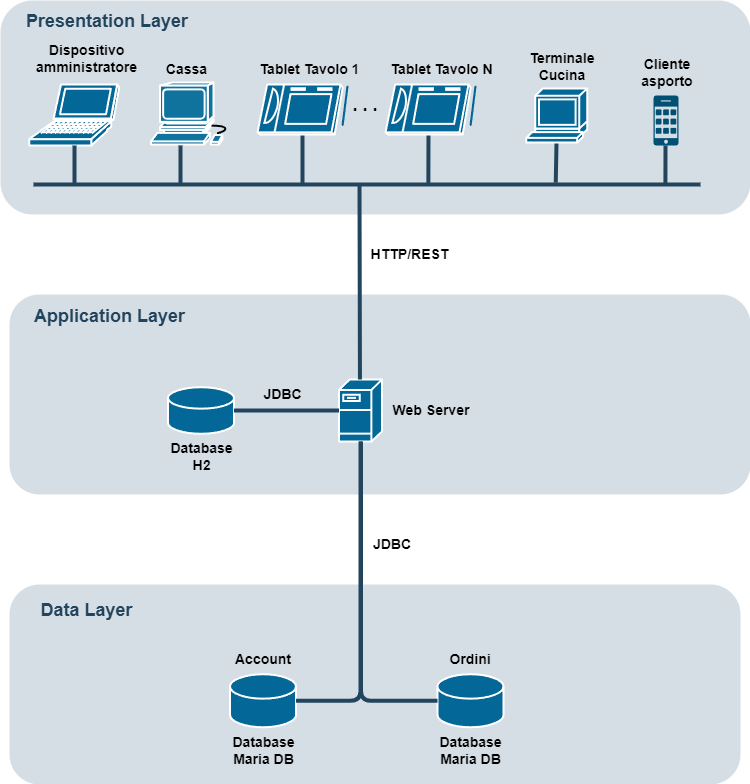
\includegraphics[scale=0.5]{iterazione0/images/topologia}
	\caption{Topologia del sistema\label{fig:topologia}}
\end{figure}

\clearpage